\documentclass[a4paper]{article}
    \usepackage[UTF8]{ctex}
    \usepackage{amsmath,amsthm,amssymb}

    \usepackage{minted}
    \usepackage{xcolor}
    \usepackage[colorlinks,linkcolor=red,anchorcolor=blue,citecolor=green]{hyperref}
    \usepackage[margin=1in]{geometry}
    \usepackage{caption}
    \usepackage{graphicx}
    \usepackage{subfigure}
    \usepackage{float}
    \usepackage{fontspec}
    \usepackage{booktabs}
    \setmainfont{Times New Roman}
    \setmonofont{Consolas}
    \definecolor{bg}{rgb}{0.9,0.9,0.9}
    \usemintedstyle{manni}
    \setminted{
    linenos,
    autogobble,
    breaklines,
    breakautoindent,
    bgcolor=bg,
    numberblanklines=false,
    }

\begin{document}
    \begingroup
    \hypersetup{linkcolor=black}
    \tableofcontents
    \endgroup
    \newpage
    \section{项目介绍}
        \subsection{想法来源}
初入学交大,在开学典礼以及各种班会、讲座上,我被推荐了许许多多的重要的网站:教务处网站,学生办网站,生活园区网站等等.
这些网站对于身处交大的学生而言,每一个都含有必需且重要的信息,所以我不得不常常去浏览,以免错过某些通知公告.

诚然,可以使用RSS订阅的方法来解决这个问题,事实上,我也是这么做的. 但除此之外, 有时候需要查看过往的通知, 而这些网站
的搜索功能往往难以使用,或者根本就形同虚设;至于使用百度等通用搜索引擎,由于其时效性与针对性不强,用起来也颇有不便.

因此, 在构思本课程的大作业项目时, 我决定做一个针对交大的文本搜索引擎,用以检索校内信息. 

而关于多媒体信息检索,考虑到校内的图片大多数为各种活动的新闻照片,其中的主体是交大的师生们,我便萌生了做一个人脸搜索引擎的想法,
可以找出一个人在哪些照片中出现.
        \subsection{基本思路}
本项目主要分为两部分:文本搜索与人脸搜索.

对于文本搜索,首先爬取一定数量的相关网页并存储在本地,对其进行数据处理,使用
ElasticSearch创建索引并实现检索功能;对于人脸搜索,从文本搜索的保存的网页中,提取一定数量的图片并存储在本地,
剔除不含有人脸存在的图片后,对每张图片,检测其中的人脸并生成特征向量,在检索时,匹配相似度达到阈值的图片.

    \newpage
    \section{实现过程}
        \subsection{数据爬取}
在本课程前期的上机实验中,我已经实现了基本的爬虫、解析工具类,在此便可以直接使用. 其具有的多线程爬取,线程池,
编码自动检测,BloomFilter等功能,在之前的实验报告中已较详细地说明,这里就不再展开.

值得一提的是,在进行本项目的过程中,我实现了一些新的功能:爬取范围限定,网页的动态优先级.

爬取范围限定,即是将爬取的网页限定在一定的范围内.本项目中,我限定仅爬取交大主页与新闻网,以及电院相关的部分网站的内容.
至于编程实现,采用的是最朴素的暴力匹配,尽管效率较低,但在爬虫应用中,程序的主要耗时在于网络通信,故简单的暴力匹配已经足够.
\begin{minted}{python}
    def __check_domain(self, url):
        if not self.domains:
            return True
        current_domain = urlparse(url).netloc
        return any(current_domain.find(x) != -1 for x in self.domains)
\end{minted}

网页的动态优先级,在初始时,所有域名的优先级都为100,而每次爬取时,从优先级队列中,取出优先级最大的网页,
将该网页对应的域名优先级降低10,添加其外链进入优先级队列,同时将其余所有域名的优先级提升1.编程实现的主要
代码如下:

\begin{minted}{python}
domain_to_priority[urlparse(url).netloc] -= 10
for k in domain_to_priority.keys():
    domain_to_priority[k] = min(100, domain_to_priority[k] + 1)
\end{minted}

这样的操作,可以确保爬取网页的顺序相对均匀,避免出现在一段时间内只爬取某一网站的现象,对爬取对象而言,
也能一定程度减轻其压力,实现爬虫的友善性.

至于图片数据的爬取,在完成对网页数据的爬取之后,从网页内容中提取出\mintinline{html}{img}标签对应的
图片地址,将其下载保存至本地即可.这一步骤较为简单,故在此不详述.

        \subsection{数据预处理}
在完成数据的爬取之后,面对约10k的数据量,在对其进行索引操作之前,我先做了一些预处理工作,清理无用数据,以便后续工作.

对于网页数据,由于在爬取时我并没有严格的检查爬取内容是否为HTML文档,实际爬取的数据中含有少量的非HTML文档(比如Word文档与
PDF文件),以及一些错误页面(比如404页面).这些数据会干扰后续的索引与检索工作,因此需要被清理.

对于非HTML文档,分析爬取的网页,我发现某些特定的URL是文件下载链接,那么,只需要从爬取的网页数据中,找到这些URL对应的数据,
将其清理即可;对于无意义的错误页面,其主要特征在于文件大小很小(往往小于2kb),那么也很容易将其发现.
\begin{minted}{python}
import os
total = 0
valid = 0
file_to_remove = []
with open("..\\data\\index.txt", mode="r") as original_index:
    with open("..\\data\\new_index.txt", mode="w") as new_index:
        for line in original_index:
            total += 1
            try:
                url, file = line.split()
            except:
                continue
            if not os.path.exists(file):
                continue
            to_remove = url.find("fileUpload.action") != -1 or url.find("download.action") != -1
            to_remove = to_remove or os.path.getsize(file) <= 2048:
            if to_remove:
                file_to_remove.append(file)
                continue
            new_index.write("{}\t{}\n".format(url, file))
            valid += 1
print("{}/{}".format(valid, total))
confirm = input("There are {} invalid files, remove all?".format(len(file_to_remove)))
if confirm and confirm[0].lower() == 'y':
    for file in file_to_remove:
        os.remove(file)
    print("All removed.")
\end{minted}

对于图片数据,在后续步骤中,我将检测其中的人脸并提取特征,为了减少后续的工作量,需要对图片进行粗筛,去除那些明显不含有
人脸的图片.在这一步,准确度和速度的权衡中,速度更为重要,因此我使用传统的机器学习方法,用OpenCV进行特征匹配:

\begin{minted}{python}
import cv2
import sys
import os

faceCascade = cv2.CascadeClassifier("haarcascade_frontalface_default.xml")

total, face_exist = 0, 0
images_with_faces = list()

data_dir = "..\\data"
image_dir = os.path.join(data_dir, "image_data")
image_index = os.path.join(data_dir, "image_index.txt")
new_image_index = os.path.join(data_dir, "new_image_index.txt")

with open(image_index, mode="r") as i_index:
    with open(new_image_index, mode="w") as new_i_index:
        for line in i_index:
            try:
                image_url, image_file, page_url, html_file = line.split()
            except:
                continue
            total += 1
            gray_img = cv2.imread(os.path.join(image_dir, image_file), cv2.IMREAD_GRAYSCALE)
            gray_img = cv2.equalizeHist(gray_img)
            faces = faceCascade.detectMultiScale(
                gray_img,
                scaleFactor=1.1,
                minNeighbors=5,
                minSize=(10, 10)
            )
            if len(faces) > 0:
                print("\n{img}".format(img=image_file))
                face_exist += 1
                new_i_index.write(
                    "{}\t{}\t{}\t{}\n".format(
                    image_url, image_file, page_url, len(faces)))
            print("\r{}/{}".format(face_exist, total), end="")
\end{minted}
        \subsection{数据索引}
对于网页数据的索引,本课程之前的上机实验中,采用的是Lucene,而在本项目中,我使用了ElasticSearch,一个基于Lucene的
更高层次抽象,抛弃了繁冗的细节,使用时更加简便.同时在性能上,也显著优于直接使用Lucene.编程实现的主要代码:
\begin{minted}{python}
class HtmlDoc(Document):

    title = Text(analyzer="ik_max_word", search_analyzer="ik_smart")
    url = Keyword()
    host = Keyword()
    text = Text(analyzer="ik_max_word", search_analyzer="ik_smart")

    class Index:
        name = "qianmo"
        settings = {
            "number_of_shards": 2,
        }

connections.create_connection(hosts=['localhost'])
HtmlDoc.init()
indexed_num = 0
with open(index_file, mode="r", encoding="utf8") as f:
    for line in f:
        url, file_path = line.split()
        file_path = os.path.join(data_dir, file_path)
        with open(file_path, mode="r") as html_file:
            html_content = html_file.read()
        text = html_to_text(html_content)
        title = get_title(html_content, url)
        host = urlparse(url).netloc
        doc = HtmlDoc(title=title, text=text, url=url, host=host)
        doc.save()
        indexed_num += 1
\end{minted}

可以看出,ElasticSeach创建索引的过程较为简单方便.至于上面代码中调用的函数,相较于之前的上机实验,
我也做了一些针对性的改进,但简洁起见,不在此贴出其具体实现.

对于图片数据的索引,先从每张图片中提取出可能的多个人脸,然后为每个人脸生成特征向量并保存.在上一步的数据预处理中,
我采用的是OpenCV中传统的特征匹配方法,而在此,为了更高的提取精度,我使用了MTCNN\cite{zhang2016joint}与FaceNet\cite{schroff2015facenet}.

MTCNN\cite{zhang2016joint}主要有3个网络结构:Proposal Net(P-Net), Refine Net(R-Net), Output Net(O-Net),
可以实现图片中较为精确地人脸检测与定位. 在本项目中,对其输入一张可能存在人脸的图片,其输出为多个矩形框选中的人脸,

FaceNet\cite{schroff2015facenet}是Google的研究人员提出的一种深度学习人脸检测模型,可以将一人脸映射为欧式空间中的
固定维度向量. 在本项目中,对其输入一张人脸,则得到一个512维的人脸特征向量.

在实际创建索引时,由于本项目中含有的人脸数在15k左右,在运行FaceNet模型时,需要设定合理的批尺寸(Batch size).如果批尺寸过大,
运行时会出现OOM错误;而如果批尺寸过小,则总的运行时间会很长.批尺寸需要合理权衡,最终我设定为1k.

需要说明的是,这一部分的代码我参考了Github上FaceNet的开源实现
\footnote{Face recognition using Tensorflow: https://github.com/davidsandberg/facenet}
,并使用了其给出的训练好的模型.由于这部分的代码较长,简洁起见,在此不贴出,源代码已随报告附上.
        \subsection{数据检索}
对于网页数据,其索引与检索都是借助于ElasticSearch实现.那么,实现网页数据的检索相对而言就十分简单了,并且,
还可以轻松地实现关键词高亮功能.
\begin{minted}{python}
def search_html(query_string, page=1, page_size=10):
    search_from = page_size * (page - 1)
    index = "qianmo"
    doc_type = "doc"
    fields = ["title", "text"]
    tick = time.time()
    response = es.search(
        index=index,
        doc_type=doc_type,
        body={
            "query": {
                "multi_match": {
                    "query": query_string,
                    "fields": fields
                }
            },
            "from": search_from,
            "size": page_size,
            "highlight": {
                "pre_tags": ["<span class = \"highlight\">"],
                "post_tags": ["</span>"],
                "fields": {
                    "title": {
                        "no_match_size": 100  
                    },
                    "text": {
                        "fragment_size": 25,
                        "number_of_fragments": 4,
                        "no_match_size": 100
                    }
                }
            }
        }
    )
    tock = time.time()
    time_used = tock - tick
    result_num = response["hits"]["total"]
    search_result = list()
    for hit in response["hits"]["hits"]:
        single_result = dict()
        single_result["title"] = hit["highlight"]["title"][0]
        single_result["content"] = "...".join(hit["highlight"]["text"])
        single_result["url"] = hit["_source"]["url"]
        search_result.append(single_result)
    result_data = {
        "time_used": time_used,
        "total_num": result_num,
        "page": page,
        "search_result": search_result,
        "query_string": query_string,
    }
    return result_data
\end{minted}

\label{face_index}
对于图片数据,在索引过程中,我计算了所有图片中所有人脸的512维特征向量,并保存了每张脸对应的相关信息.那么,在查询时,
给定一张图片,需要做的就是从中定位出人脸,提取其特征向量,与已有的所有特征向量进行比对,找出相似度超过阈值的那些人脸.

需要说明的是,关于高维向量的匹配,本课程介绍了局部敏感哈希(LSH)的方法,其效率应当是高于朴素的暴力匹配.然而在本项目中,
这一点并不成立,原因在于:我用Python实现的简单LSH运行效率不如Numpy中使用C++编写的矩阵运算.因此,我最终采用的方法是:
将所有人脸的特征矩阵(N$\times$512矩阵)与目标人脸的特征向量(512维)相乘,得到相似度向量(N维),从而找出匹配人脸.
\begin{minted}{python}
def search_face(image_hash):
    result_data = dict()
    result_data["target_url"] = "/static/upload/" + image_hash+".jpg"
    result_data["search_result"] = list()
    image_file = os.path.join(upload_dir, image_hash+".jpg")
    target_feature = extract_feature(image_file)
    if target_feature is None:
        print("No face detected!")
        return result_data
    similarity = np.dot(all_faces, target_feature.T)
    sorted_index = np.argsort(similarity)
    prev_similarity = None
    for i in range(1, 21):
        if similarity[sorted_index[-i]] <= similarity_threshold:
            break
        if prev_similarity == similarity[sorted_index[-i]]:
            continue
        prev_similarity = similarity[sorted_index[-i]]
        face_info = face_info_list[sorted_index[-i]]
        image_url, page_url = face_info.split()[0], face_info.split()[2]
        page_title = get_page_title(page_url)
        result_data["search_result"].append({
            "url": image_url,
            "page_url": page_url,
            "page_title": page_title,
        })
    return result_data
\end{minted}

在上面代码中,涉及的具体函数(如\mintinline{python}{extract_feature})与索引过程类似,在此略去其具体实现.
        \subsection{网站前后端实现}
在完成了以上步骤后,整合网站的前后端.对于网页搜索,我基本沿用了本课程中期整合的前端设计,而仅仅将后端从Lucene替换为ElasticSearch;
对于人脸搜索,我做了比较大的改动.

首先是人脸检索的主页面,需要由用户上传含有人脸的图片.考虑到上传的易用性与美观性(朴素的HTML文件上传元素不够美观且难以改造),
我使用了Github上开源项目,Uppy\footnote{Uppy: https://github.com/transloadit/uppy},一个优秀的前端文件上传
插件,支持用户通过本地文件、网络文件以及摄像头来上传图片.
\begin{minted}{js}
const uppy = Uppy.Core({
  debug: false,
  autoProceed: true,
  restrictions: {
    maxFileSize: 2000000,
    maxNumberOfFiles: 1,
    minNumberOfFiles: 1,
    allowedFileTypes: ['image/*']
  }
})
.use(Uppy.Dashboard, {
  inline: true,
  target: '.DashboardContainer',
  replaceTargetContent: true,
  showProgressDetails: true,
  note: 'Only 1 image file allowed, up to 2 MB',
  height: 300,
  width:1000,
  metaFields: [
    { id: 'name', name: 'Name', placeholder: 'file name' },
    { id: 'caption', name: 'Caption', placeholder: 'describe what the image is about' }
  ],
  browserBackButtonClose: true
})
.use(Uppy.Webcam, { target: Uppy.Dashboard })
.use(Uppy.XHRUpload, { endpoint: '/image-upload' })
\end{minted}

当用户上传图片时,网站后端接收到图片,首先计算图片内容的哈希值,与已有图片进行比对,倘若存在,便不再重复保存,直接返回
哈希值即可;若不存在,则在保存后返回哈希值.而前端得到后端返回的哈希值,便直接携带哈希值前往搜索结果页面.
\begin{minted}{python}
class Upload:

    def POST(self):
        x = web.input()
        if "files[]" not in x:
            print("No file found!")
            return None
        image_content = x.get("files[]")
        md5 = hashlib.md5()
        md5.update(image_content)
        image_hash = md5.hexdigest()
        image_path = os.path.join(upload_dir, str(image_hash)+".jpg")
        if not os.path.exists(image_path):
            with open(image_path, mode="wb") as f:
                f.write(image_content)
        result_info = {
            "hash": image_hash,
        }
        web.header('content-type', 'text/json')
        return json.dumps(result_info)
\end{minted}

\begin{minted}{js}
uppy.on('upload-success', (file, resp, uploadURL) => {
    window.location.href = "/search/face/"+resp.hash;  
})
\end{minted}

而在执行搜索时,后端根据图片的哈希值,找到保存的图片,进行检索并返回结果即可,这一部分在图片数据的检索\ref{face_index}中已提及,但值得一提的
是,在未经优化之前,单张图片查询时间在30秒以上,这显然是无法接受的,因此我进行了一些简单的优化,使得最终查询时间降至500毫秒以内.

经过分析,未经优化之前,查询的主要耗时在于Tensorflow加载MTCNN以及FaceNet的模型,而在加载完成之后,计算时间相对较短,在
1秒以内.因此,我采用了预先加载模型的方法,在启动时就将完整的模型载入内存,计算时不再重复载入,这样大幅加快了查询速度.
\begin{minted}{python}
# init
es = connections.create_connection(hosts=["localhost"])
upload_dir = "static/upload"
similarity_threshold = 0.6935
graph = tf.Graph()
with graph.as_default():
    gpu_options = tf.GPUOptions(per_process_gpu_memory_fraction=0.6)
    sess = tf.Session(config=tf.ConfigProto(gpu_options=gpu_options, log_device_placement=False))
    with sess.as_default():
        pnet, rnet, onet = align.detect_face.create_mtcnn(sess, None)
        facenet.load_model(facenet_model)
\end{minted}

此外,我将人脸对应信息也预先载入内存,以空间换时间.
\begin{minted}{python}
all_faces = np.load(face_feature_file)
with open(face_info_file, mode="r", encoding="utf8") as f:
    face_info_list = f.readlines()
\end{minted}

在经过这样的优化之后,人脸搜索的查询时间在1秒左右.更进一步的优化在于,将部分信息放入ElasticSearch,查询时借助ElasticSearch,
代替原先的顺序查找.以查询图片对应的网页标题为例:
\begin{minted}{python}
def get_page_title(page_url):
    index = "qianmo"
    doc_type = "doc"
    response = es.search(
        index=index,
        doc_type=doc_type,
        body={
            "query": {
                "term": {
                    "url": page_url,
                }
            }
        }
    )
    result_num = response["hits"]["total"]
    if result_num == 0:
        return "未找到标题"
    return response["hits"]["hits"][0]["_source"]["title"]
\end{minted}

至此,优化基本完成,查询时间可控制在500毫秒以内.
而搜索结果的前端展示,我实现了瀑布流效果,同时在每张图片上增加了悬停遮罩,显示图片相关信息与链接.具体效果参见成果展示\ref{face_demo}.
    \newpage
    \section{成果展示}
        \subsection{文本搜索}
\begin{figure}[H]
\centering

\includegraphics[width=\textwidth]{image/html1.png}
\caption{网页搜索主页面}
\end{figure}
\begin{figure}[H]
\centering
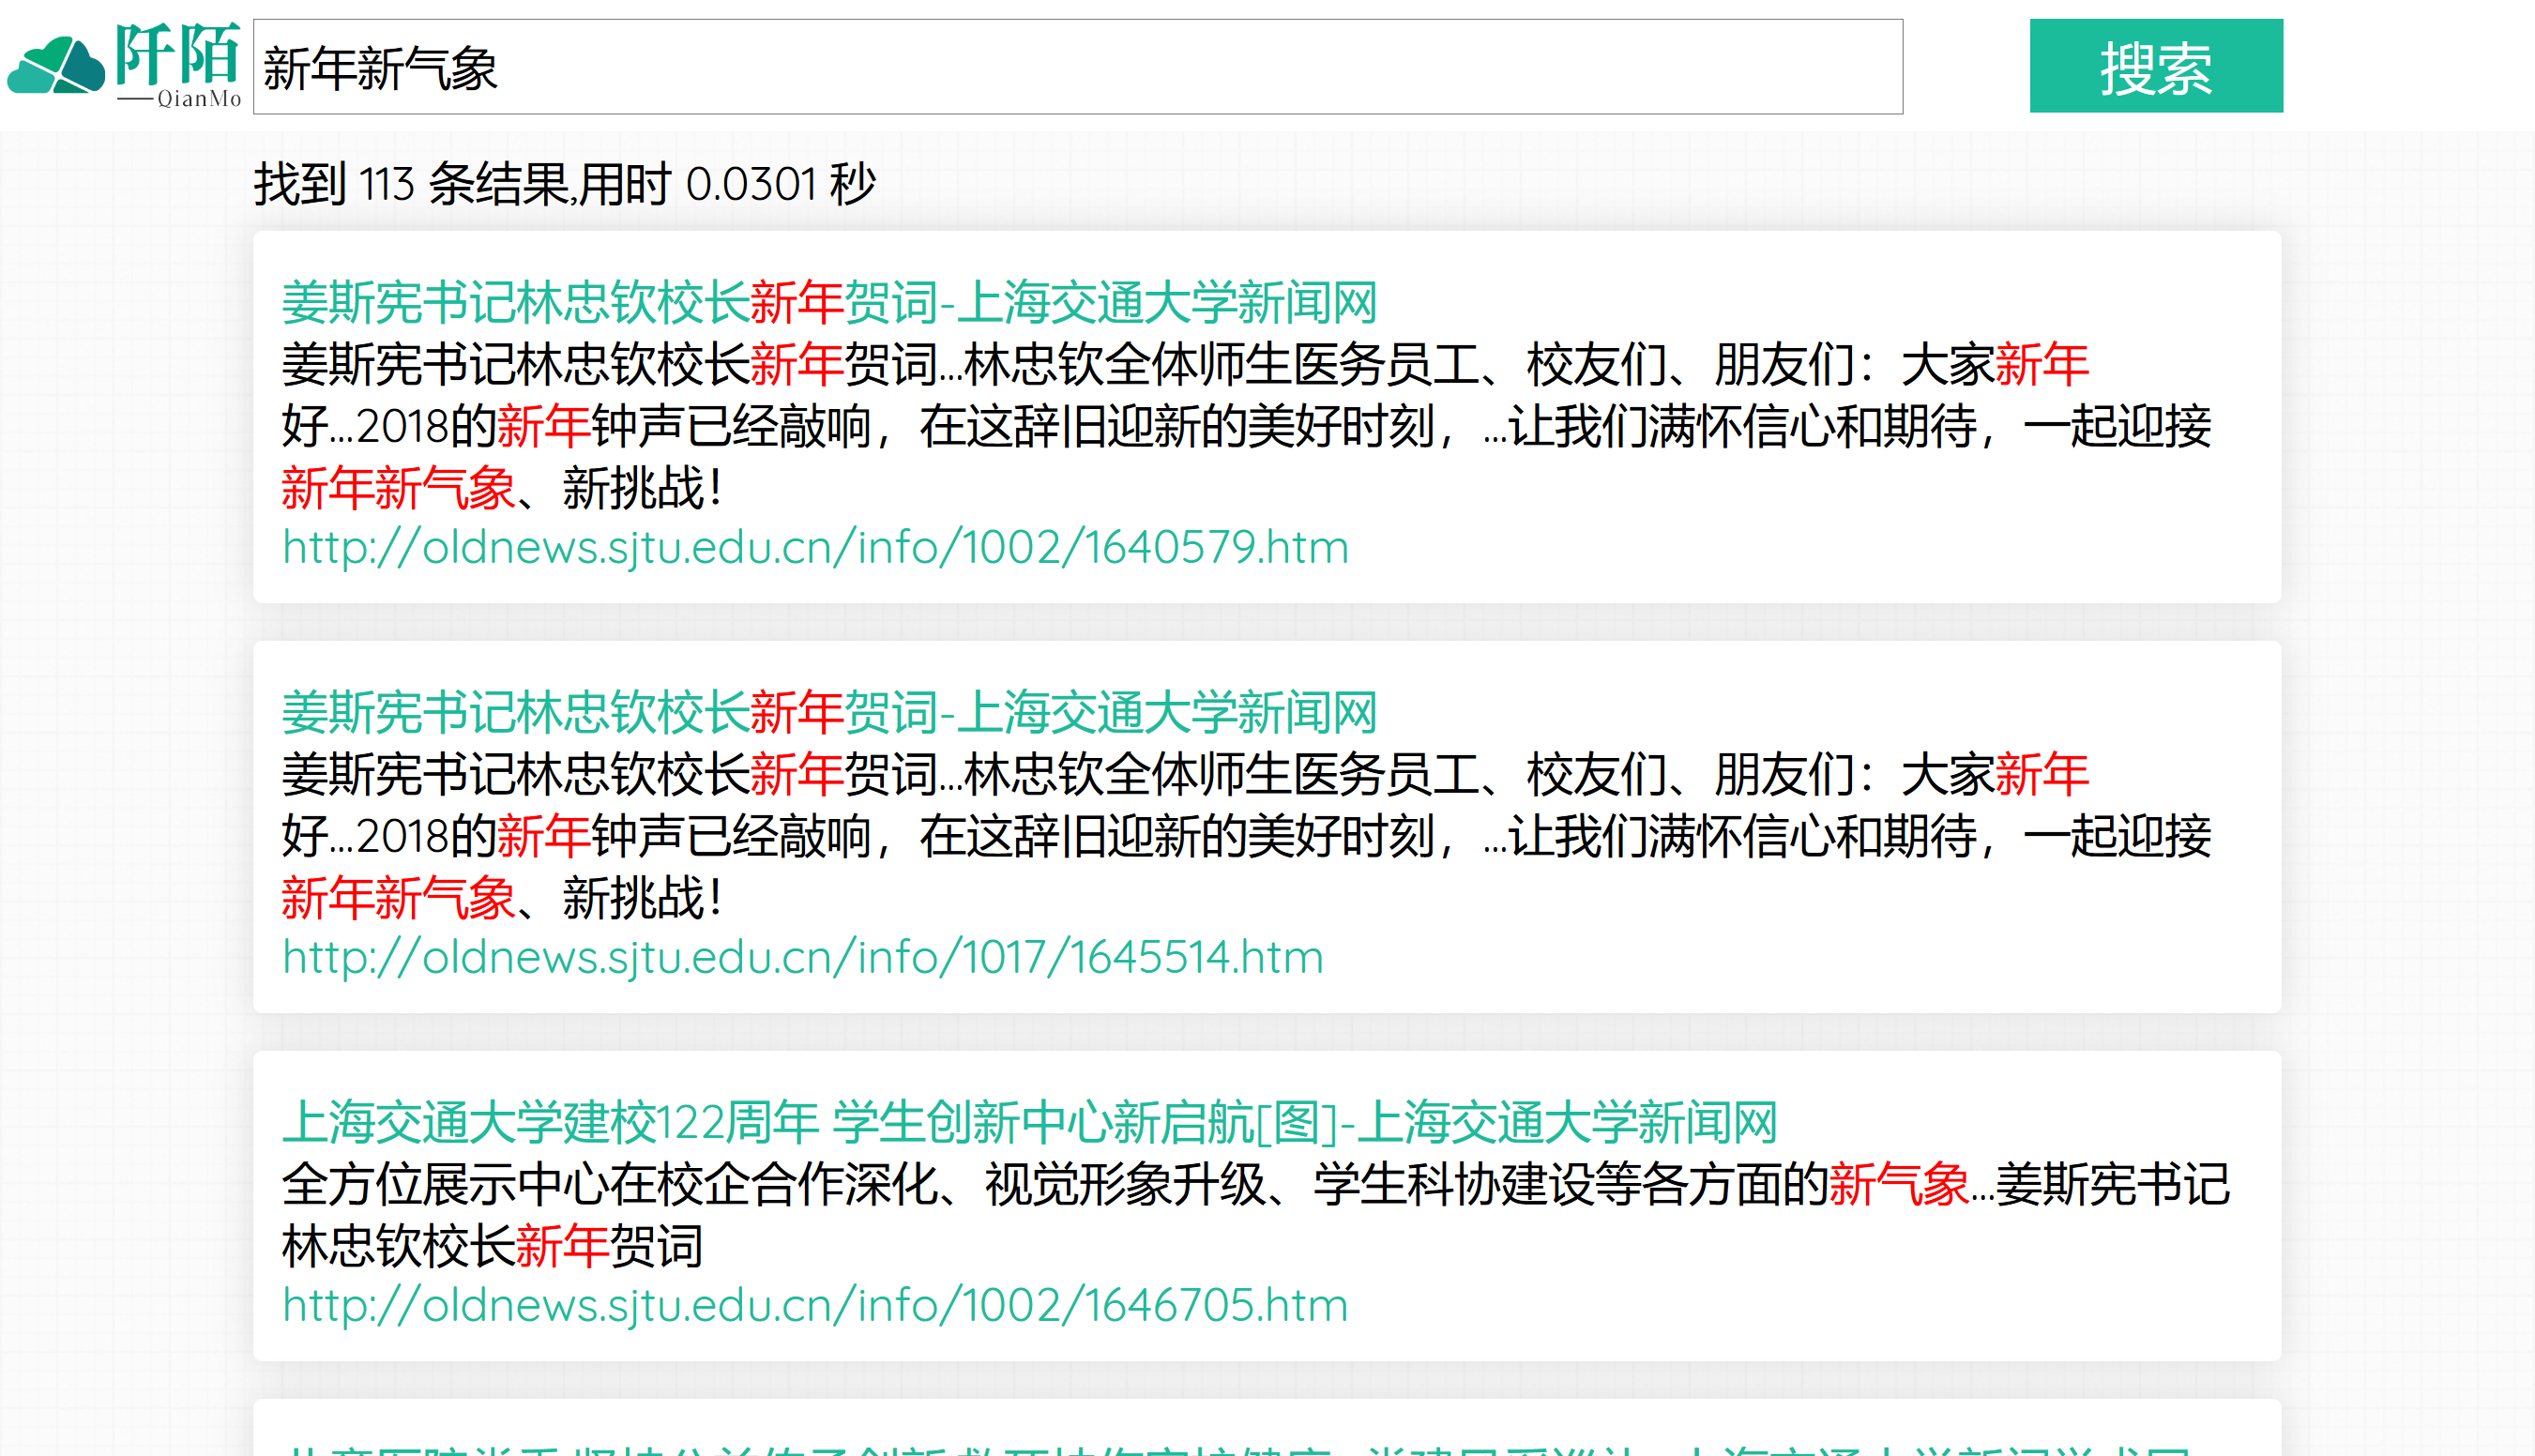
\includegraphics[width=\textwidth]{image/html2.png}
\caption{网页搜索结果页面}
\end{figure}
\begin{figure}[H]
\centering
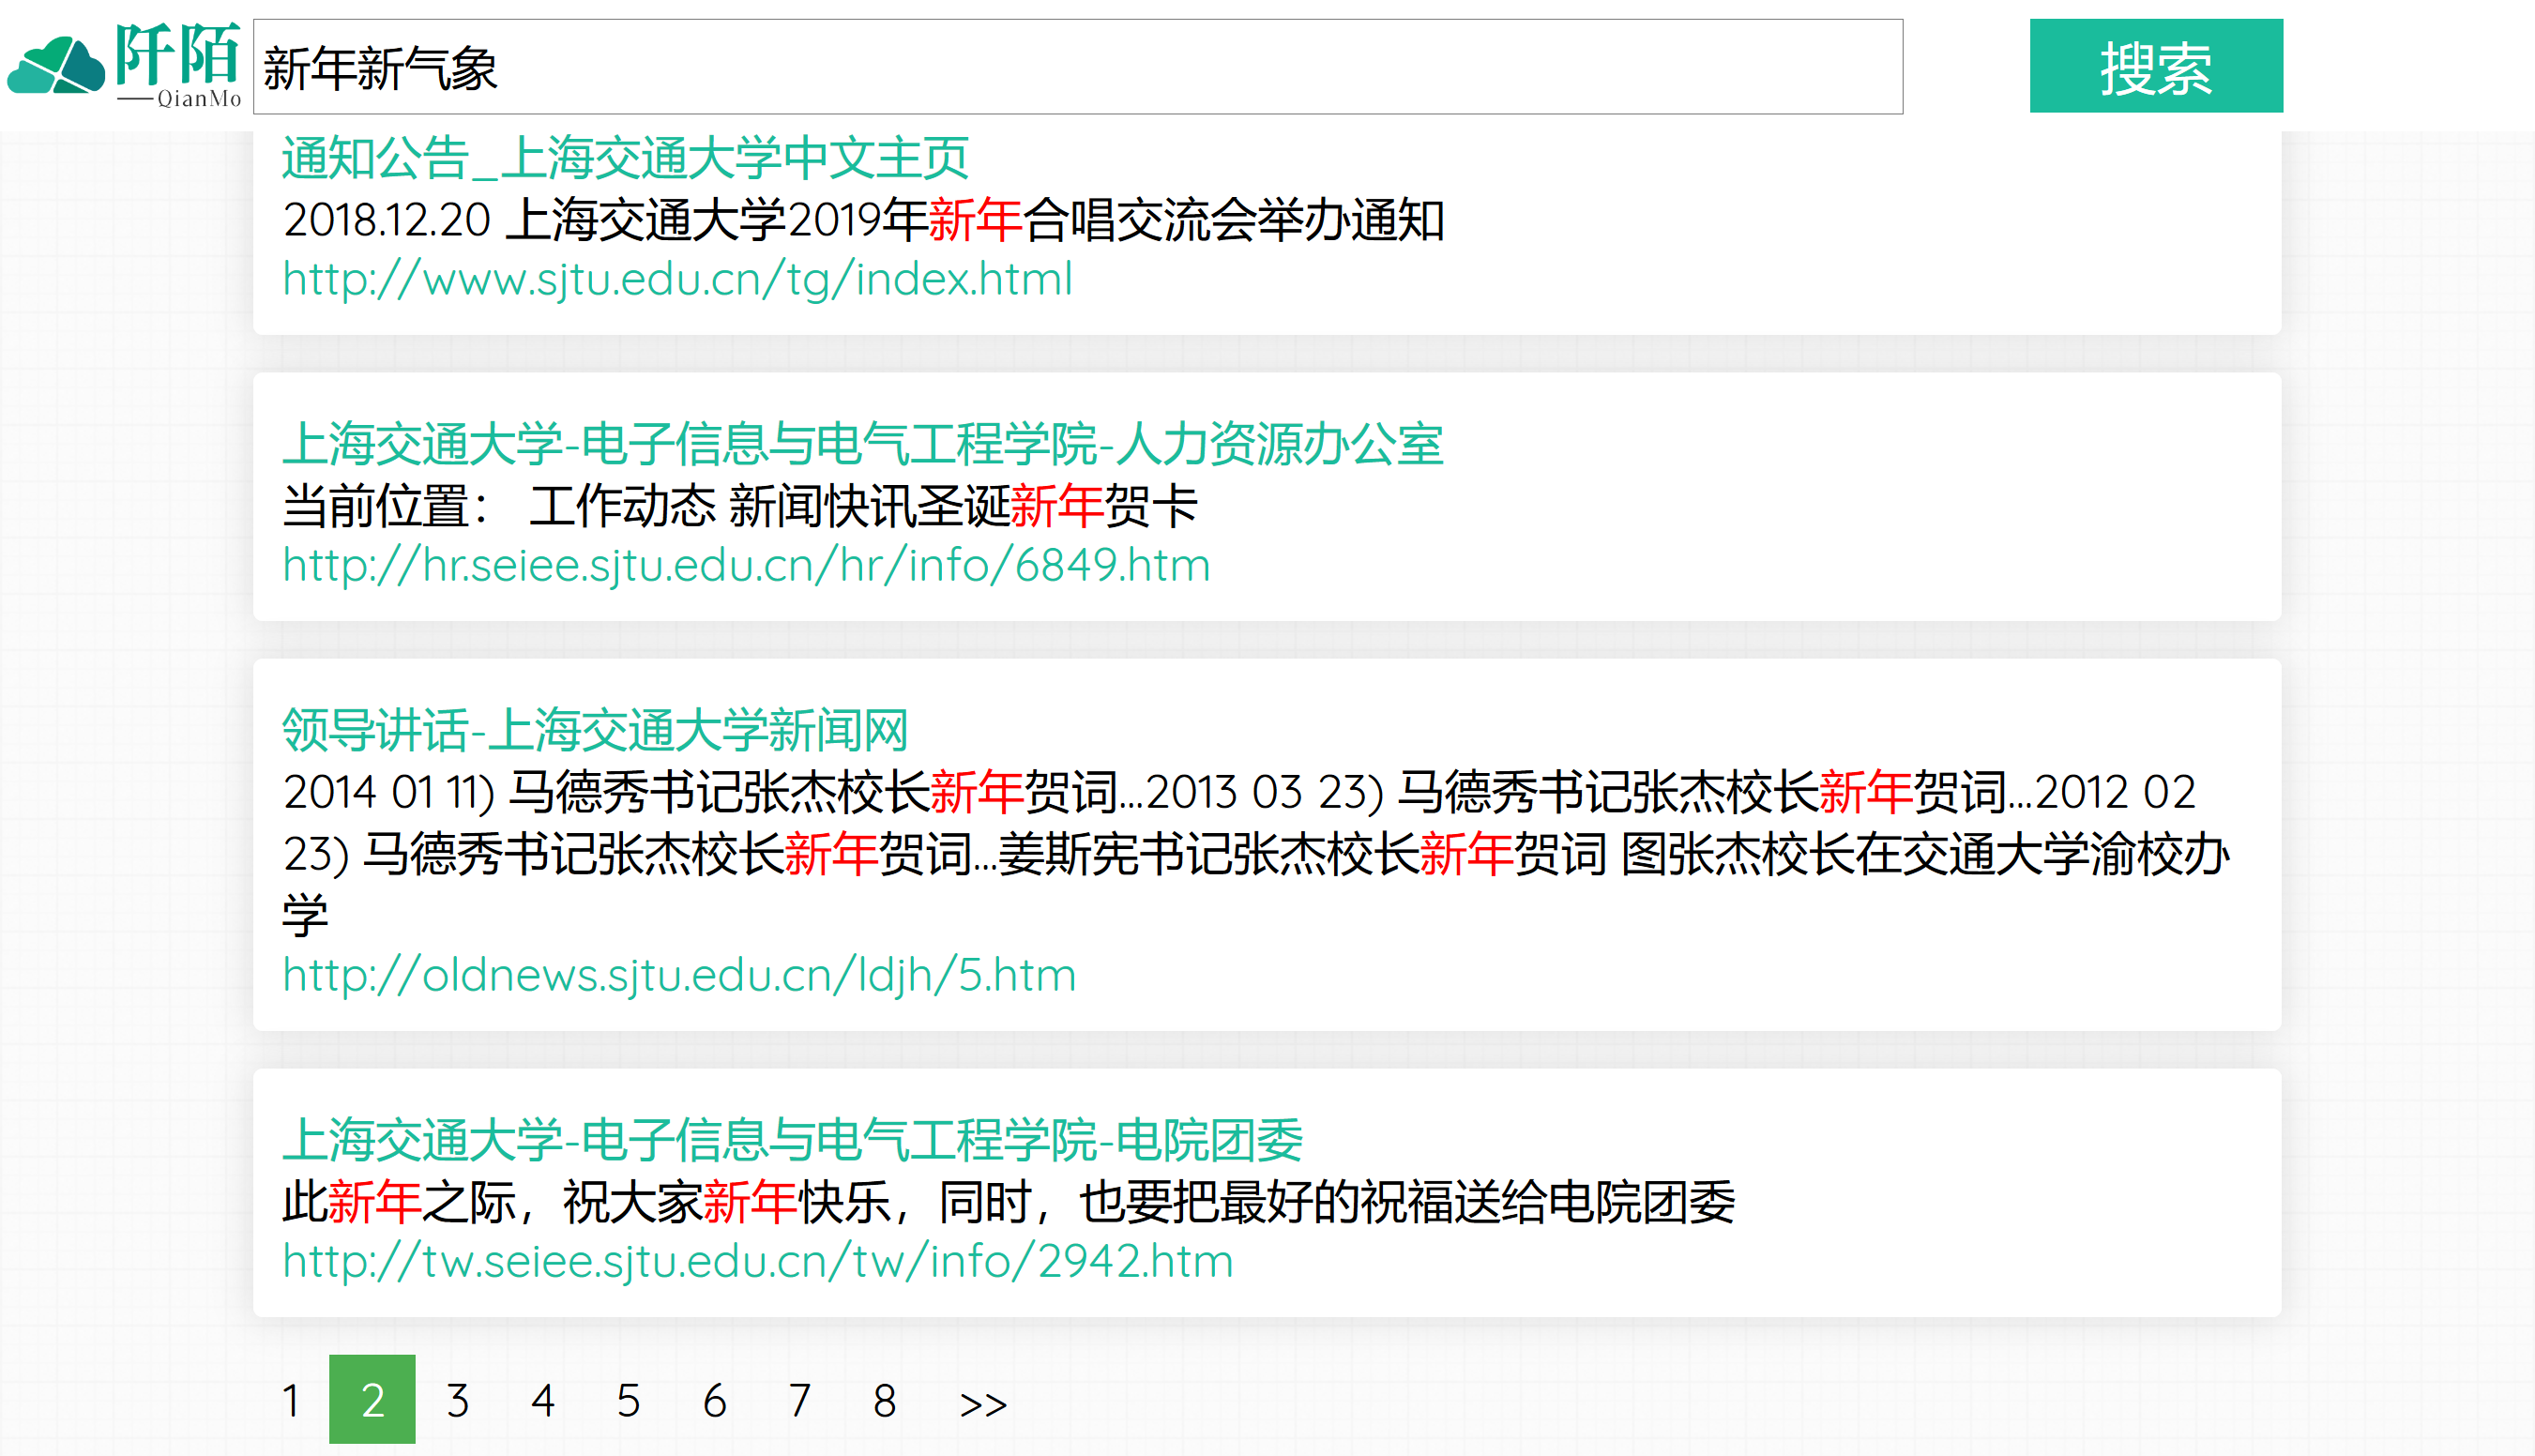
\includegraphics[width=\textwidth]{image/html3.png}
\caption{网页搜索结果页面}
\end{figure}
        \subsection{人脸搜索}
        \label{face_demo}
\begin{figure}[H]
\centering
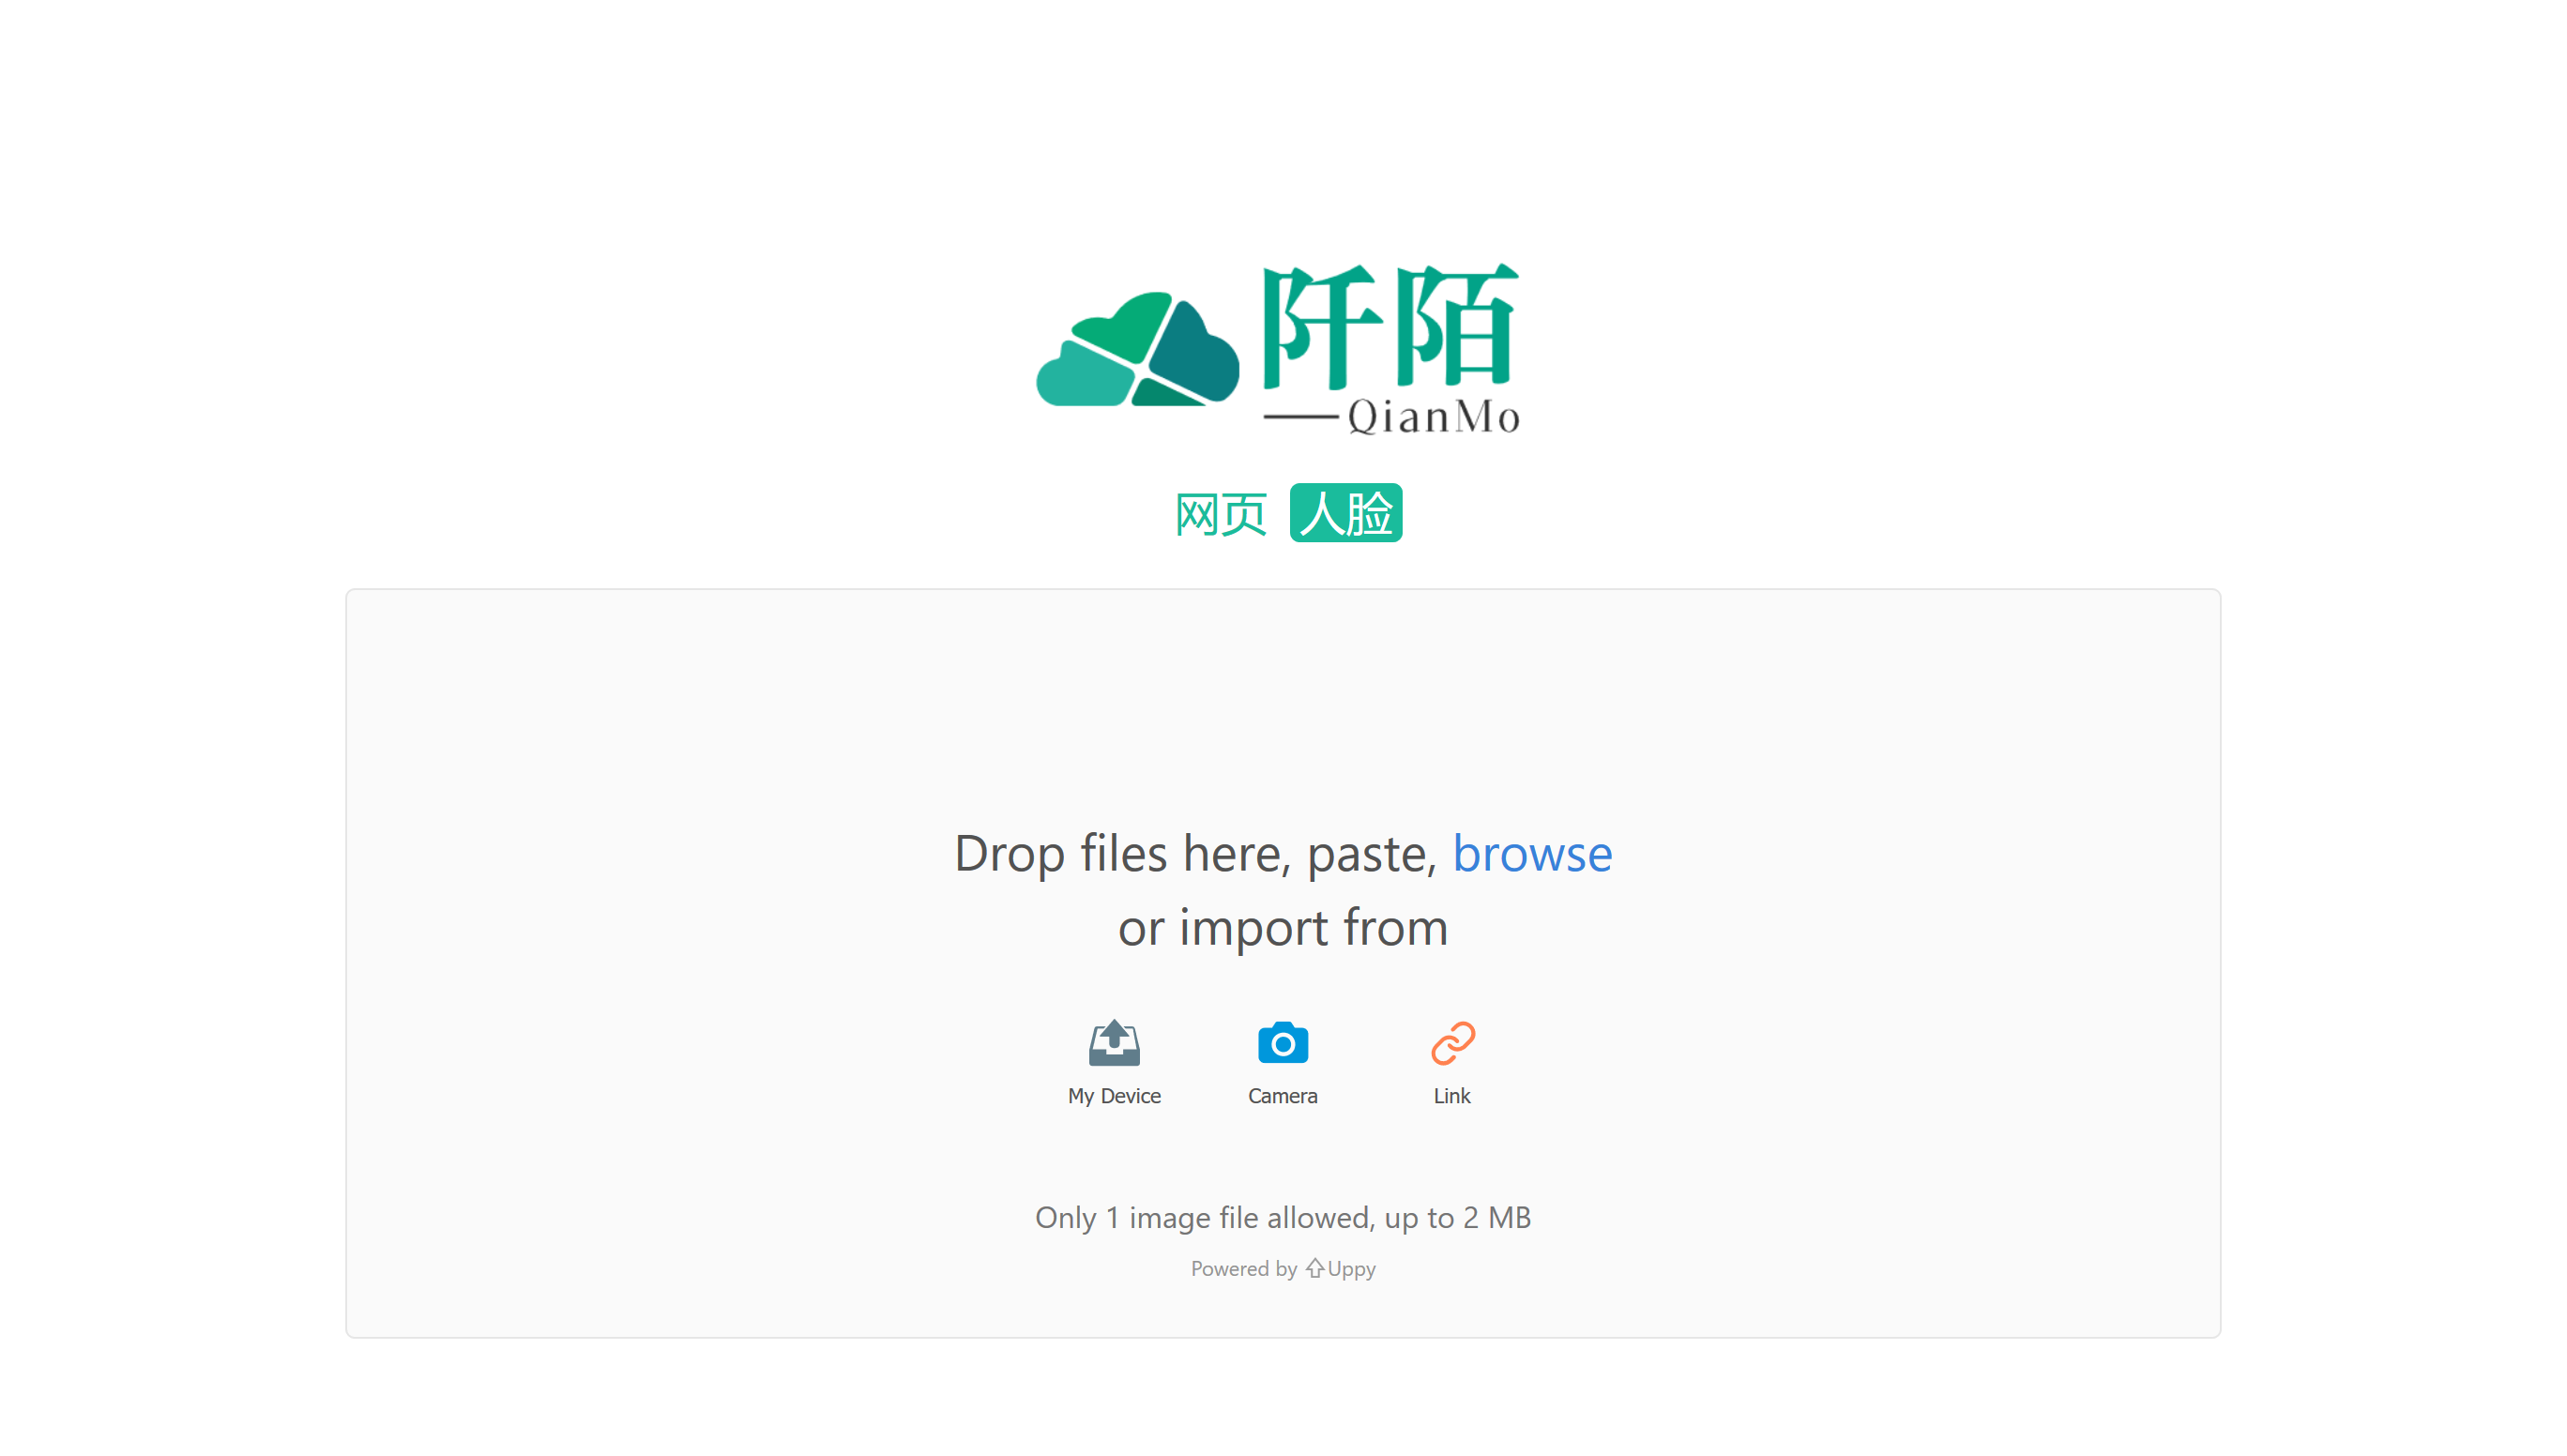
\includegraphics[width=\textwidth]{image/face1.png}
\caption{人脸搜索主页面}
\end{figure}
\begin{figure}[H]
\centering
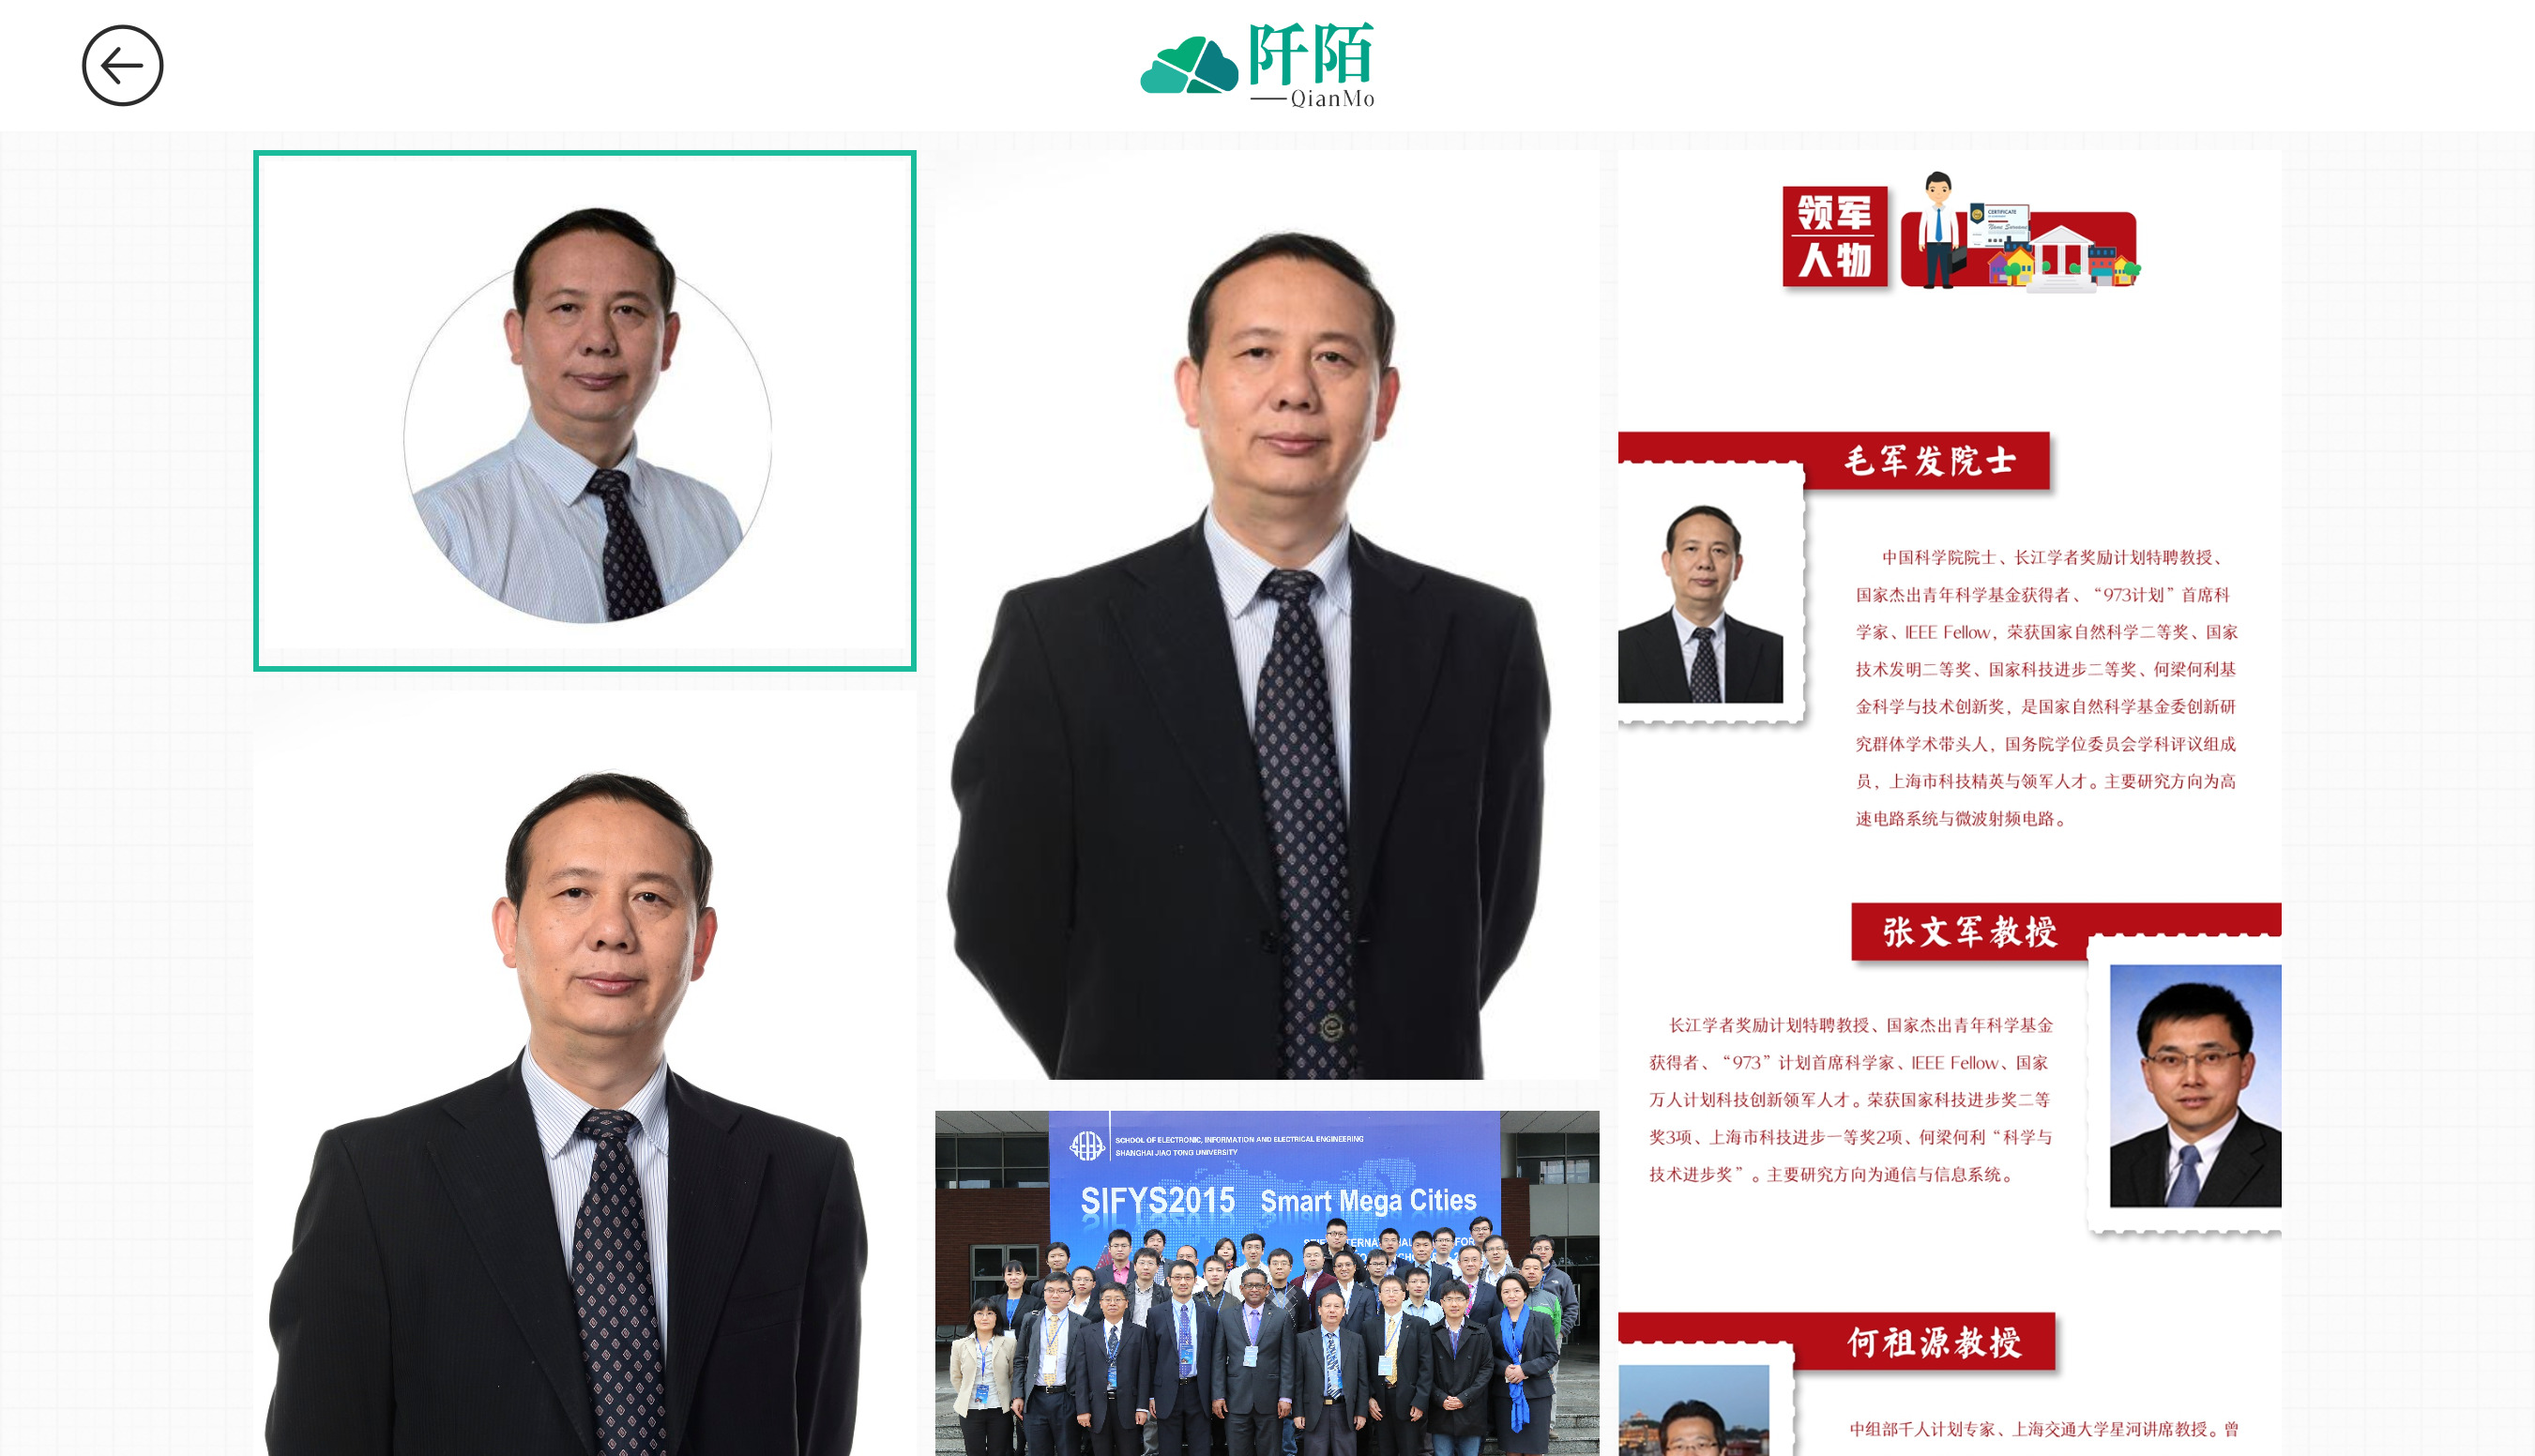
\includegraphics[width=\textwidth]{image/face2.jpg}
\caption{人脸搜索结果页面(绿色边框图片为目标图片)}
\end{figure}
\begin{figure}[H]
\centering
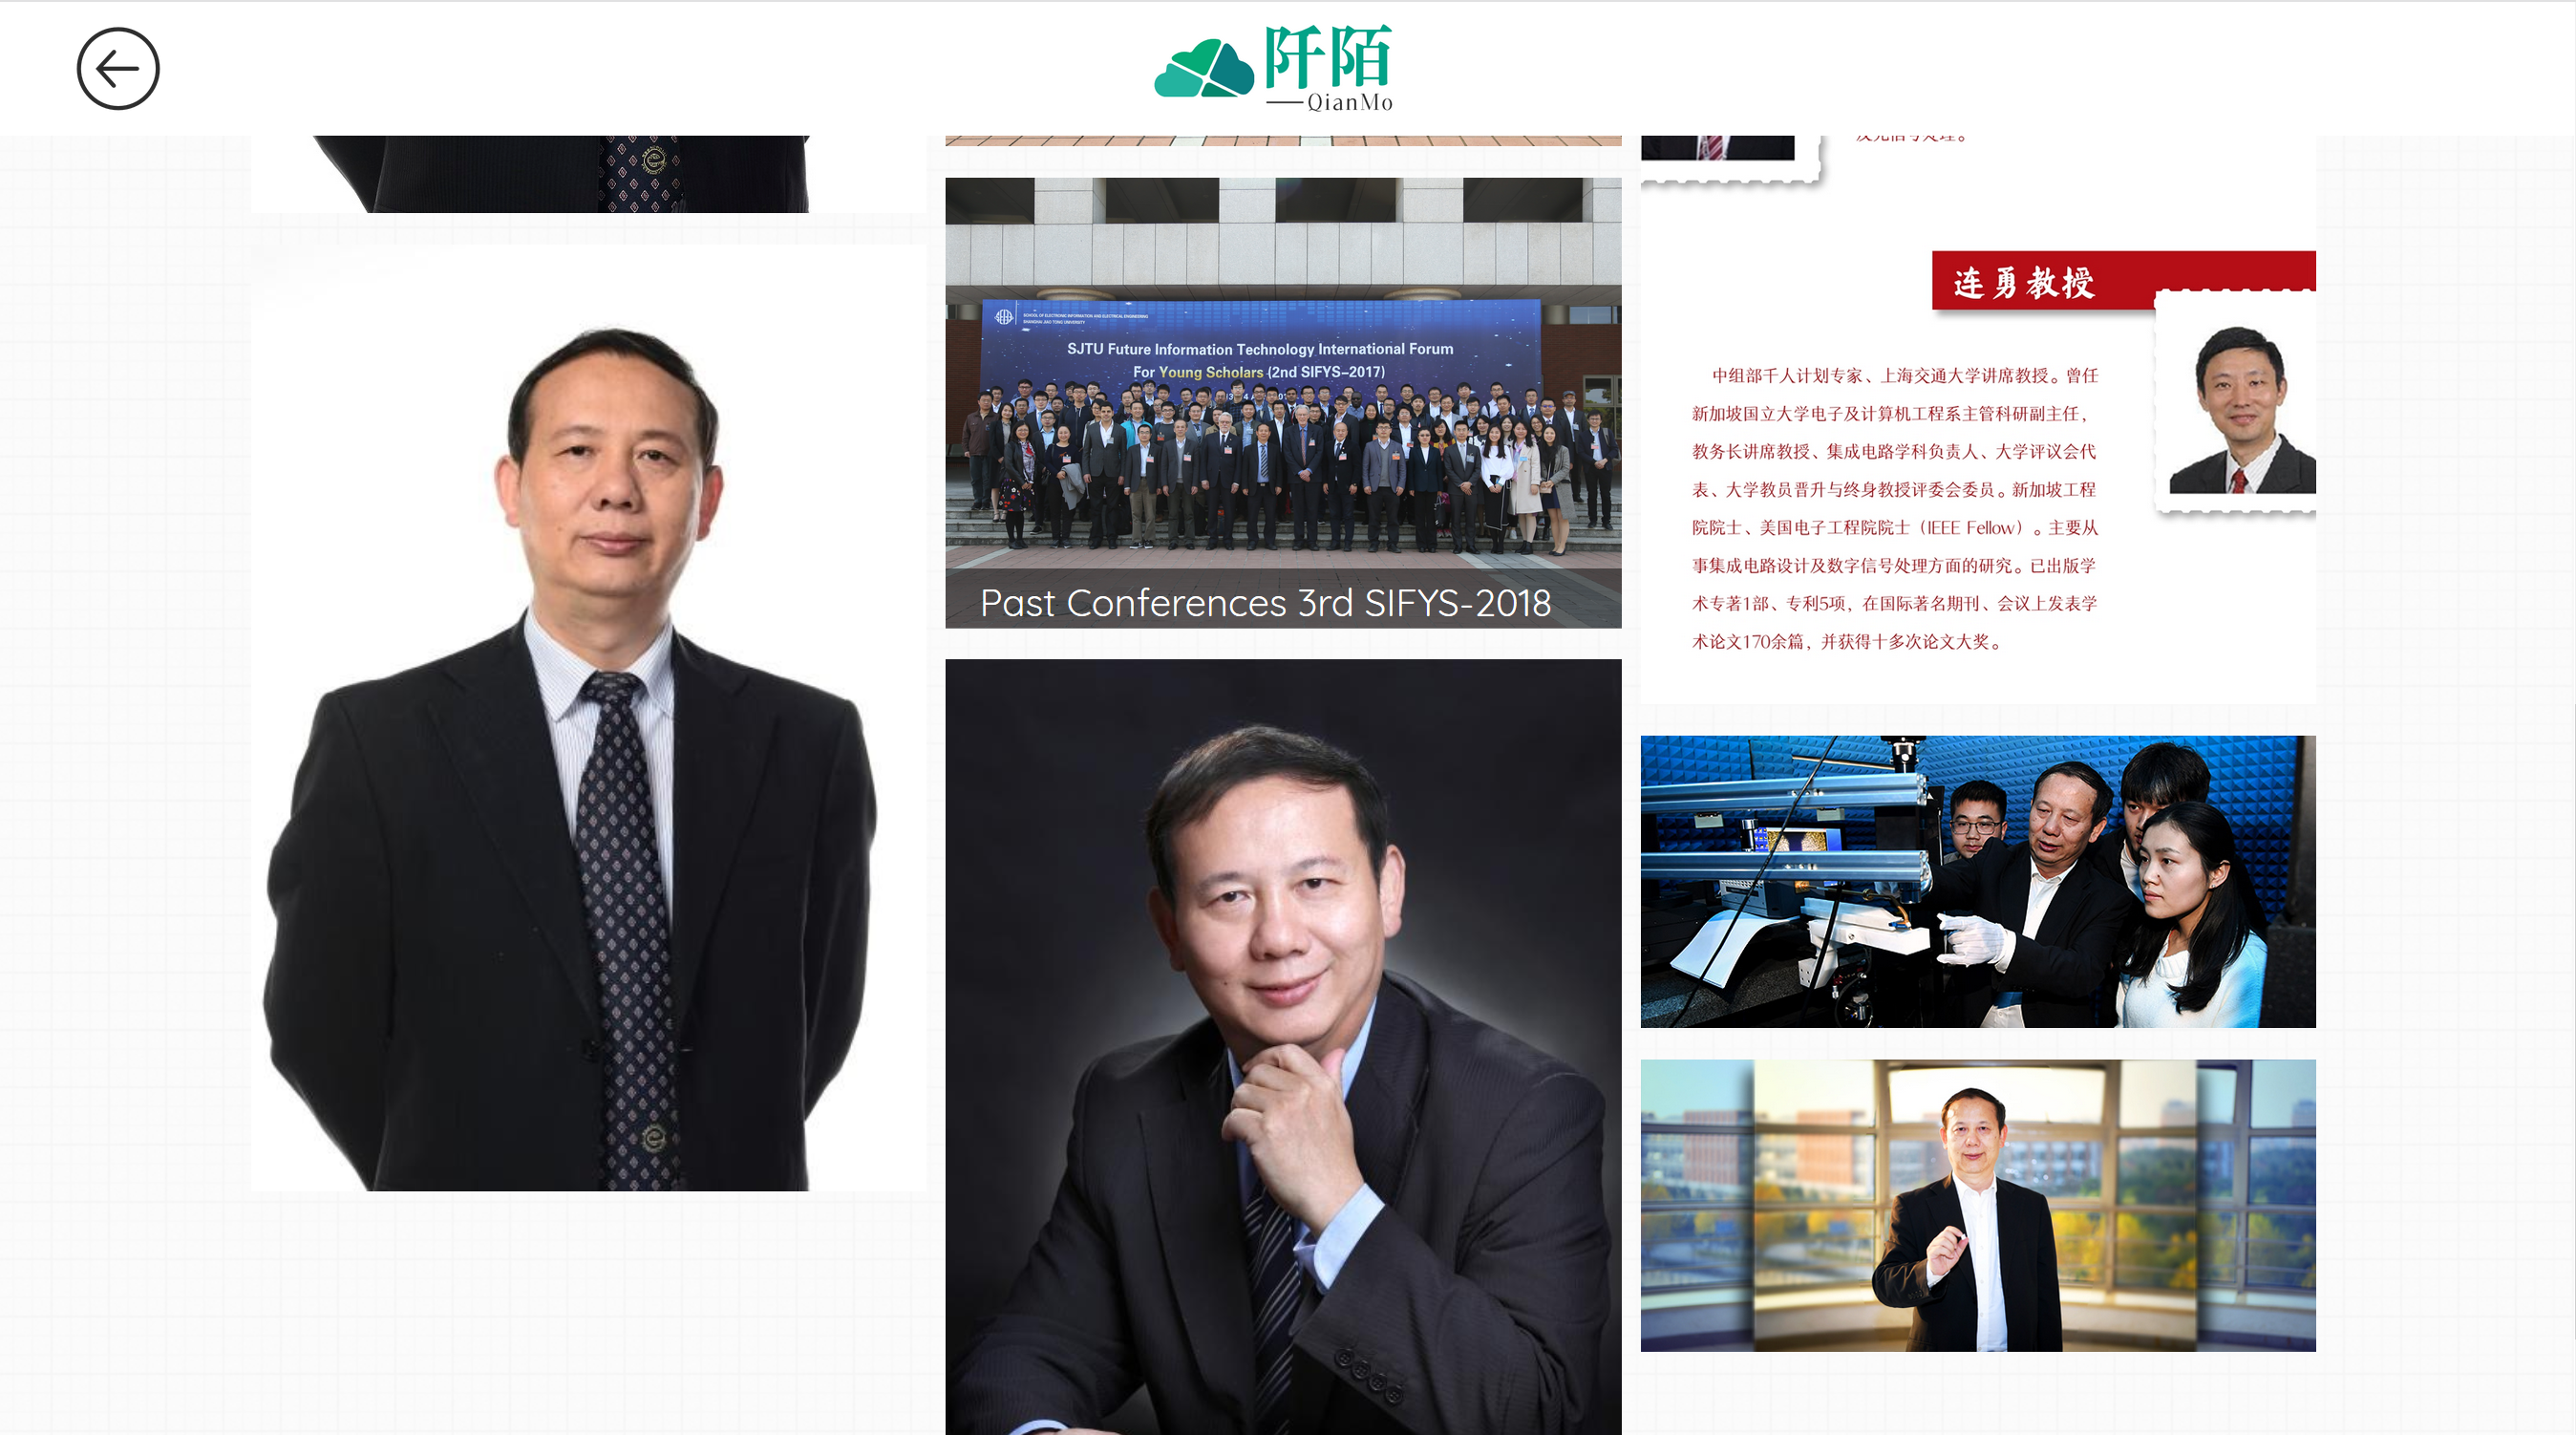
\includegraphics[width=\textwidth]{image/face3.png}
\caption{人脸搜索结果页面}
\end{figure}
    \newpage
    \section{总结与分析}
在本项目中,我综合运用了本学期所学的多媒体检索相关知识,同时结合深度学习相关知识,实现了一个简单的校内信息
检索引擎.在这一过程中,我学习了ElasticSearch的基本概念以及使用方法,并将传统的计算机视觉方法与深度学习方法
综合使用,收获颇丰.当然,除此之外,在网站开发的前后端,我都有新的收获,如何优化后端性能与美化前端.

关于一个人独立完成本项目,比起多人协作,诚然显得有些突兀.但在我看来,多人的协作是存在沟通成本的,包括代码的耦合与
思路的耦合.那么,对于一个课程的大作业,总的工作量其实并不是很大,在单人可以完成且不会很吃力的范畴内,多人协作
甚至可能会导致效率的降低,因而我选择了
独自完成本项目.此外,这也给了我同时接触完整的项目的机会,包括信息的爬取与处理,网站的前端与后端,可以更加全面地
锻炼自己的能力,我觉得是很有收获的.

    \newpage
    \bibliographystyle{plain}
    \bibliography{reference}
\end{document}
